\documentclass{beamer}
\usepackage[utf8]{inputenc}
\usepackage{graphics}
\mode<presentation> {
\usetheme{unc}}
\setbeamertemplate{navigation symbols}{} % To remove the navigation symbols from the bottom of all slides uncomment this line

\usepackage{graphicx} % Allows including images
\usepackage{booktabs} % Allows the use of \toprule, \midrule and \bottomrule in tables


\usepackage{hyperref}
\hypersetup{linkcolor=blue,colorlinks=true}


% Remove symbols
\beamertemplatenavigationsymbolsempty


%\usetheme{default}

\usefonttheme{serif}

%----------------------------------------------------------------------------------------
%	TITLE PAGE
%----------------------------------------------------------------------------------------


\title[The Puzzle of War (II)]{\LARGE{The Puzzle of Interstate War, Part II: Information and Commitment Problems}}
\author[POLI 150]{Steven Saroka}
\institute{POLI 150}
\date{Jan. 30 - 1 Feb. 2024}


\begin{document}

\begin{frame}
\titlepage % Print the title page as the first slide
\end{frame}

\begin{frame} 
	\frametitle{\LARGE{Class}}
	\begin{itemize}
		
			\item Fearon (1995) Review

			\item Incomplete Information Explanation for War

			\item Credible Communication

			\item Limits of the Incomplete Information Explanation
			\item Credible Commitments

			\item Issue Indivisibility

			\item Example: South China Sea

			\item Is War Obsolete?
		
	\end{itemize}
\end{frame}

\begin{frame} 
	\frametitle{\LARGE{Central Questions}}
	\begin{center}
		\LARGE How can incomplete information and incentives to misrepresent it lead to war within the bargaining model of war? How can commitment problems and indivisibility lead to war? 
	\end{center}
\end{frame}

\begin{frame} 
	\frametitle{\LARGE{Key Terms}}
	\begin{itemize}
		\item Incomplete Information 
		\item Incentives to Misrepresent
		\item Credible Communication
		\item Costly Signaling
		\item Costly Signaling Strategies
		\item Commitment Problem 
		\item Credible Commitment
		\item Preventive War
		\item Preemptive War
		\item Indivisibility
	\end{itemize}
\end{frame}

\begin{frame} 
	\frametitle{\LARGE{Fearon Review}}
	Group yourselves and answer the following:
	\begin{itemize}
		\item What was Fearon's main point?
		\item What does Fearon identify as the ``central puzzle" of war?
		\item What are the 5 incorrect bargaining explanations for war that Fearon critiques?
		\item What are the 3 bargaining explanations for war that Fearon identifies?
	\end{itemize}
\end{frame}

\begin{frame} 
	\frametitle{\LARGE{Fearon Review}}
	What was Fearon's main point? \pause
	\begin{itemize}
		\item At time of writing (1995), (neo)realist explanations for war all had problems. \pause
		\item Fearon criticizes some for lacking logical validity, while arguing others are not empirically supported. This means there may not be a rationalist explanation for war. \pause
		\item As a rationalist explanation for war is a key part of realism, a threat to one is a threat to the other. \pause
		\item Fearon's article is thus an attempt to solve this problem.
	\end{itemize}
\end{frame}

\begin{frame} 
	\frametitle{\LARGE{Fearon Review}}
	What does Fearon identify as the ``central puzzle" of war? \pause
	\begin{itemize}
		\item ``[War] is costly and risky, so rational states should have incentives to locate negotiated settlements that all would prefer to the gamble of war" but existing theories fail to identify why they do not settle (380).
	\end{itemize}
\end{frame}

\begin{frame} 
	\frametitle{\LARGE{Fearon Review}}
	 What are the 5 incorrect bargaining explanations for war? \pause
	\begin{enumerate}
		\item Anarchy. \pause Rebuttal: War is still costly, so what about anarchy prevents negotiation?
		\\~\\
		\item Preventive war. \pause Rebuttal: why can't the rising power make concessions to avoid costly war?
		\\~\\
		\item Positive expected utility of war. \pause Rebuttal: War is always a gamble with a chance of losses.
	\end{enumerate}
\end{frame}

\begin{frame} 
	\frametitle{\LARGE{Fearon Review}}
	What are the 5 incorrect bargaining explanations for war? 
	\begin{enumerate}
		\setcounter{enumi}{3}
		\item Disagreements over relative power (and thus over the possible outcomes of war). \pause Rebuttal: why can't states just tell each other this private information?
			\\~\\
		\item Miscalculation of opponent's willingness to fight. \pause Rebuttal: why can't states just tell each other this private information too?
	\end{enumerate}
\end{frame}

\begin{frame} 
	\frametitle{\LARGE{Fearon Review}}
	What are the 3 bargaining explanations for war that Fearon identifies? \pause
	\begin{enumerate}
		\item Private information and incentives to misrepresent it.
		\item Commitment problems. These include: \pause
		\begin{itemize}
			\item Preemptive wars
			\item Preventive wars
			\item Strategic territory/appeasement
		\end{itemize}
		\item Indivisibility
	\end{enumerate}
\end{frame}

\begin{frame} 
	\frametitle{\LARGE{Incomplete Information Basics}}
	\begin{itemize}
		\item Remember from last class that, given a divisible good and costs to war, there always exists a bargaining range. \pause
		\item \textbf{Given the existence of a bargaining range, there is always some deal that both sides would prefer to war.} \pause
		\item \textbf{Why do states choose war, given the existence of both the costs of war and the existence of a deal that both sides prefer to war?}
	\end{itemize}
\end{frame}

\begin{frame} 
	\frametitle{\LARGE{Incomplete Information Basics}}
	\begin{itemize}
		\item We can reframe this puzzle in terms of information. \pause
		\item Why can't each side calculate what the costs $c$ are for both sides, and/or the potential outcome $x$, and thereby find the bargaining range? \pause
		\item If we assume \textbf{incomplete information}, each side only knows its own costs $c$ with certainty. Each side must guess at the other's costs as well as the outcome. \pause
		\item So, what's preventing each side from simply telling the other its costs and figuring out the outcome?
	\end{itemize}
\end{frame}

\begin{frame} 
	\frametitle{\LARGE{Incentives to Misrepresent}}
	\begin{itemize}
		\item \textbf{Incentives to misrepresent incomplete information always exist.} \pause
		\item If one actor can get the other to believe that their costs are lower than they truly are, or that the outcome of the conflict will be more favorable for them than it truly is, they gain an advantage in crisis bargaining and can try to secure a better negotiated settlement for themselves. \pause
		\item However, each side is a rational actor and knows this. What does this mean?		
	\end{itemize}
\end{frame}

\begin{frame} 
	\frametitle{\LARGE{Incentives to Misrepresent}}
	\begin{itemize}
		\item \textbf{Neither side can afford to trust the other, even if they are both telling the truth.} \pause
		\item This is similar to a Prisoner's Dilemma, where cooperation is analogous to telling the truth and defection analogous to bluffing. \pause
		\item However, the problem here is not that they cannot communicate, but that they cannot trust any communication.	 \pause
		\item We say that this communication lacks \textbf{credibility}.
	\end{itemize}
\end{frame}

\begin{frame} 
	\frametitle{\LARGE{Incentives to Misrepresent}}
	\begin{itemize}
		\item This is the core of the information explanation for war: 
		\begin{itemize}
			\item Neither side can credibly communicate their private information.
			\item This means one or both are unable to propose a settlement within a bargaining range that is acceptable to both sides. \pause
			\item If each side has a different estimate for the other's $c$ and/or the outcome $x$ of the war, this can lead disagreement over the location of bargaining ranges. \pause
			\item This leaves at least one side unable to propose a deal the other side views as better than war. 
		\end{itemize}
	\end{itemize}
\end{frame}

\begin{frame}{Non-Overlapping Bargaining Ranges}
	\centering
	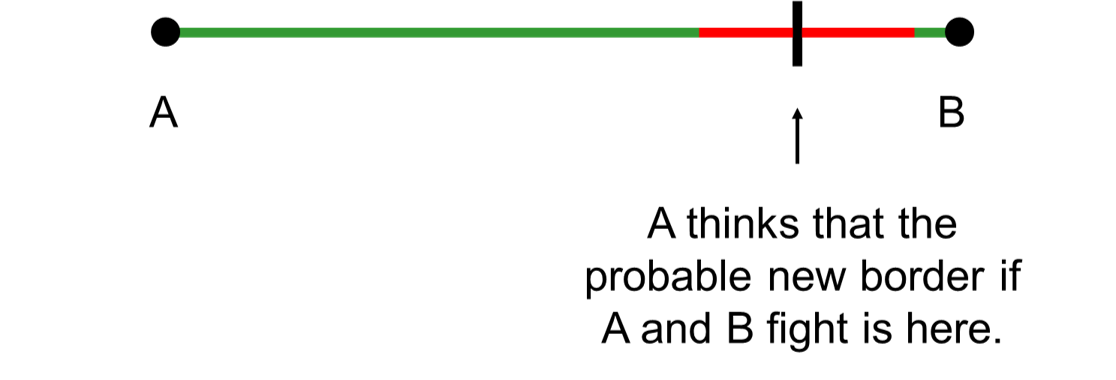
\includegraphics[width=\textwidth,height=0.8\textheight,keepaspectratio]{Bluff1.png}
\end{frame}


\begin{frame}{Non-Overlapping Bargaining Ranges}
	\centering
	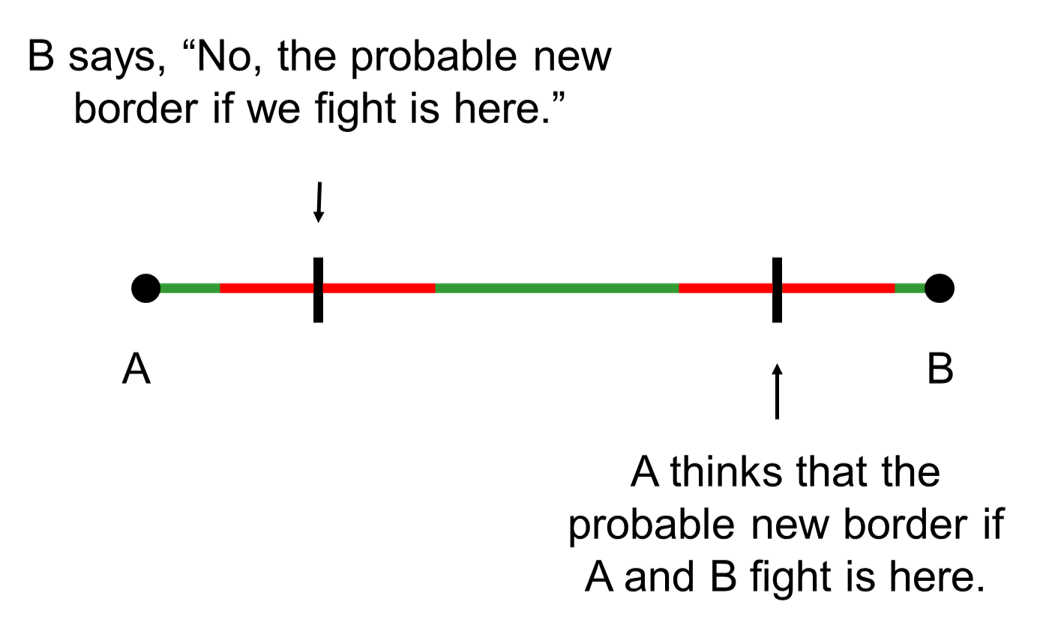
\includegraphics[width=\textwidth,height=0.8\textheight,keepaspectratio]{Bluff2.png}
\end{frame}

\begin{frame}{Non-Overlapping Bargaining Ranges}
	\centering
	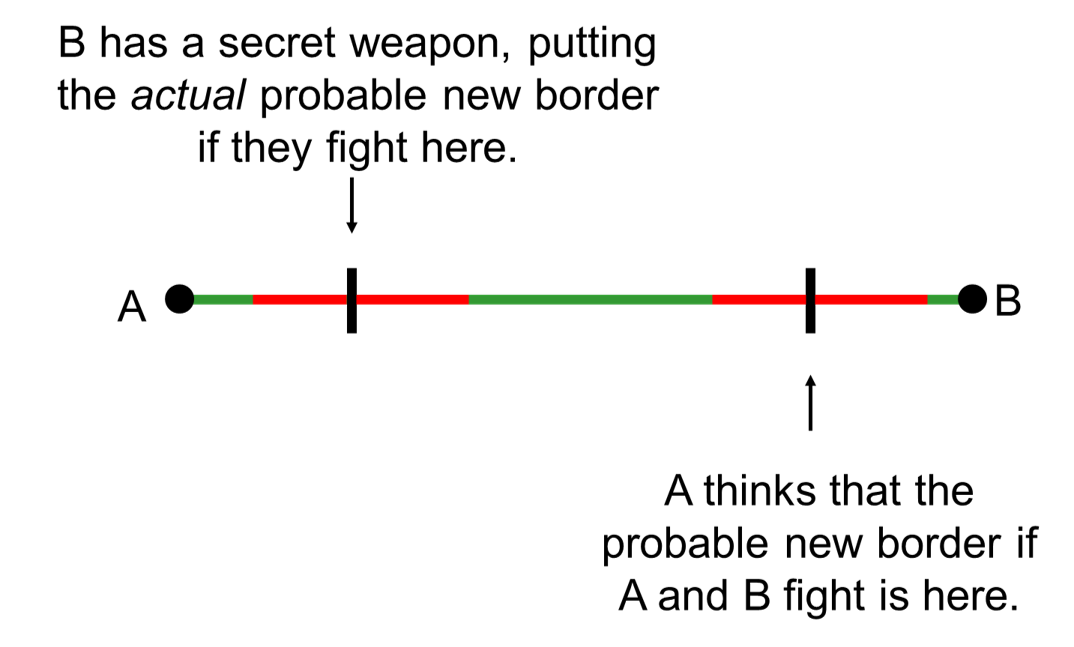
\includegraphics[width=\textwidth,height=0.8\textheight,keepaspectratio]{Bluff3.png}
\end{frame}

\begin{frame} 
	\frametitle{\LARGE{Types of Private Information}}
	\begin{itemize}
		\item So, what kinds of incomplete information do states have incentives to misrepresent? \pause
		\item Their costs $c$ and beliefs about outcome $x$, but what does that mean in the real world? \pause
		\item Costs are determined by two components: a state's \textbf{capabilities} and/or \textbf{resolve}. \pause
		\item \textbf{Capabilities}: physical ability to prevail in war (e.g. troops, arms, economic resources) \pause
		\item \textbf{Resolve}: a state's willingness to endure the costs of war to acquire a good. \pause 
		\item A state's \textbf{private information} about its own capabilities and resolve can lead to complications in bargaining.
	\end{itemize}
\end{frame}

\begin{frame} 
	\frametitle{\LARGE{Capabilities}}
	\begin{itemize}
		\item \textbf{Capabilities}: physical ability to prevail in war (e.g. troops, arms, economic resources). \pause
		\item Some capabilities are obvious or easily credibly communicated. \pause
		\begin{itemize}
			\item Number of troops on a border \pause
			\item Flashy military hardware (planes, aircraft carriers, etc.) \pause
		\end{itemize}
		\item Others are harder to credibly communicate. \pause
			\begin{itemize}
			\item Secret weapons: cannot be revealed without losing their effectiveness. \pause
			\item Intangible elements such as quality of training or morale.
		\end{itemize}
	\end{itemize}
\end{frame}

\begin{frame} 
	\frametitle{\LARGE{Types of Private Information: Resolve}}
	\begin{itemize}
		\item \textbf{Resolve}: a state's willingness to endure the costs of war to acquire a good or outcome. \pause 
		\item Resolve is even harder to communicate credibly. \pause
		\item No state's leadership or military are going to ever admit to weak resolve or armed forces prone to desertion. \pause
		\item Doubts about resolve can go both ways...
	\end{itemize}
\end{frame}

%photo and quotes from https://www.military.com/undertheradar/2015/09/21-facts-about-the-first-gulf-war
\begin{frame} 
	\frametitle{\LARGE{Resolve: Gulf War}}
	\centering
	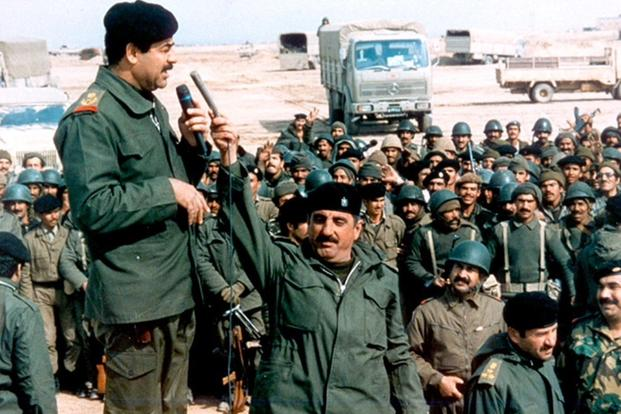
\includegraphics[width=\textwidth,height=0.63\textheight,keepaspectratio]{saddamiraqiarmy.jpg}
	\\~\\
	``Yours is a society which cannot accept 10,000 dead in one battle." \\
	\hspace*{160pt} - Saddam Hussein (1990)
\end{frame}

%photo from google
\begin{frame} 
	\frametitle{\LARGE{Resolve: Gulf War}}
	\centering
	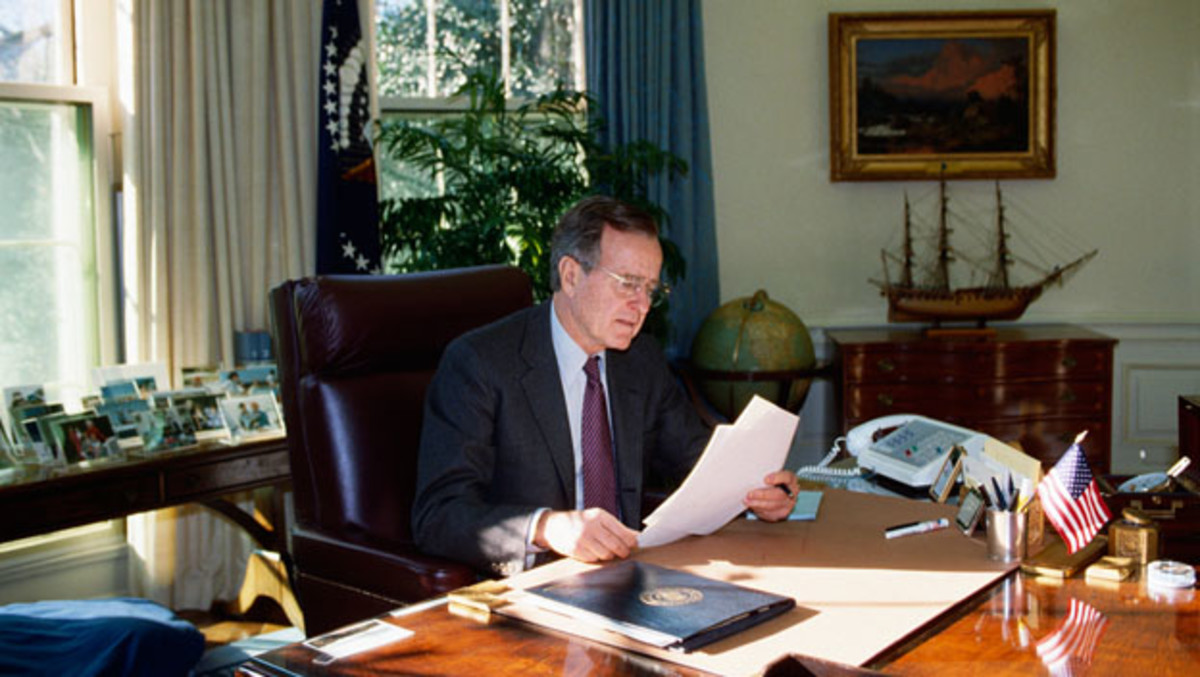
\includegraphics[width=\textwidth,height=0.7\textheight,keepaspectratio]{ghwbush.jpg}
	\\~\\
	``This will not stand, this aggression against Kuwait." \\
	\hspace*{160pt} - George HW Bush (1990)
\end{frame}

%https://www.britannica.com/event/Afghanistan-War
\begin{frame} 
	\frametitle{\LARGE{Another Example: Afghanistan}}
	Consider the case of US negotiations with the Taliban regime in Afghanistan following 9/11.
	\begin{itemize}
		\item 9/11 occurs and Al-Qaeda takes responsibility. \pause
		\item US quickly realizes AQ is being sheltered by the Taliban government of Afghanistan. \pause
		\item US demands Bin Laden and any other AQ leadership. \pause
		\item Taliban refuse but offer to put Bin Laden on trial themselves. \pause
		\item US CIA and special forces are in Afghanistan by late September, and Operation Enduring Freedom launches October 7.
	\end{itemize}
\end{frame}

\begin{frame} 
	\frametitle{\LARGE{Another Example: Afghanistan}}
What was the primary credible communication challenge here? \pause
	\begin{itemize}
		\item Taliban ultimately doubted US resolve. \pause
		\item Taliban leadership did not think US was prepared to pay the costs of a lengthy occupation. \pause
		\item US ability to win a conventional battle with the Taliban was never in doubt. \pause
		\item Taliban miscalculated by gambling that they could refuse to hand over Bin Laden, and this led to war. 
	\end{itemize}
\end{frame}

\begin{frame} 
\frametitle{\LARGE{Solutions to the Information Problem}}
\begin{itemize}
	\Large{
			\item Given these challenges, how can states effectively signal their intentions?
	}
\end{itemize}
\end{frame}

\begin{frame} 
	\frametitle{\LARGE{Solutions to the Information Problem}}
All solutions to the information problem revolve around ways to credibly communicate. These are called \textbf{costly signals}. 
	\begin{enumerate}
		\item Brinksmanship \pause
		\item Tying Hands \pause
		\item Paying for Power \pause
		\item Sunk Costs \pause
	\end{enumerate}
All of these are intended to send a \textbf{costly signal}: an action that will only be taken by a truly resolved state, and never by an unresolved state, proving credibility.
\end{frame}


\begin{frame} 
\frametitle{\LARGE{Costly Signaling: Brinksmanship}}
\begin{itemize}
	\item \textbf{Brinksmanship}: increasing the risk of accidental war to make one's threats credible. \pause 
	\item Textbook example: 1962 Cuban Missile Crisis. \pause
	\item American placement of ballistic missiles in NATO members Italy and Turkey leads to Soviet missiles being placed in Cuba. \pause
	\item Kennedy administration considers this unacceptable; both sides reach agreement to remove nuclear missiles from Cuba and Turkey after days of tension. \pause
	\item During this time, President John F. Kennedy takes steps that make nuclear war more likely, such as putting missile crews on alert. \pause
	\item This is a negotiating tactic to pressure the Soviets to dismantle nuclear missile sites in Cuba. 
\end{itemize}
\end{frame}

\begin{frame}
	\frametitle{\LARGE{Costly Signaling: Brinksmanship}}
	\centering
	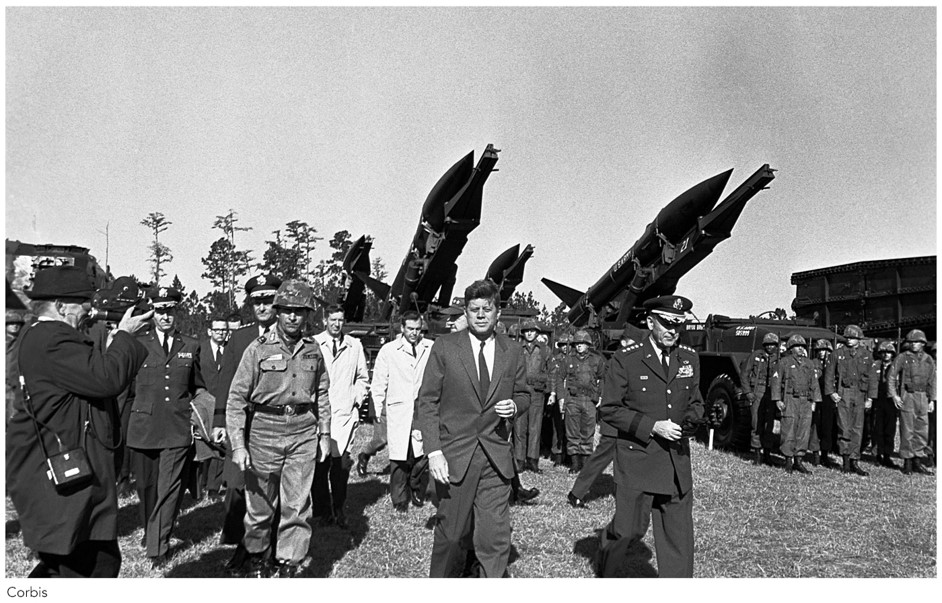
\includegraphics[width=\textwidth,height=0.8\textheight,keepaspectratio]{Cubanmissilecrisis.jpg}
\end{frame}


\begin{frame} 
\frametitle{\LARGE{Costly Signaling: Tying Hands}}
\begin{itemize}
		\item \textbf{Tying hands}: taking actions that make backing down more difficult. \pause
		\item How do states do this? By invoking \textbf{audience costs}: public commitments or threats that, once made, are damaging politically to renege on. \pause
		\item To successfully tie one's hands, the audience costs of not keeping that commitment must be greater than the costs of following through on that commitment. 
\end{itemize}
\end{frame}

\begin{frame}
\frametitle{\LARGE{Audience Costs}}
Who imposes audience costs? \pause
\begin{itemize}
	\item International audiences: any state with whom the current state might bargain in the future.
	\item Domestic audiences: voters, political opponents, etc. \pause
	\begin{itemize}
		\item Arguably more credible when coming from democracies, as voters can easily impose audience costs during an election cycle.
	\end{itemize}
\end{itemize}
\end{frame}

\begin{frame}
	\frametitle{\LARGE{Costly Signaling: Tying Hands}}
	\centering
	\includegraphics[width=\textwidth,height=0.8\textheight,keepaspectratio]{obamaredline.jpg}
\end{frame}


\begin{frame} 
	\frametitle{\LARGE{Costly Signaling: Paying for Power}}
	\begin{itemize}
		\item \textbf{Paying for power:} taking costly steps to increase one's military capabilities. \pause
		\item The resources spent in this way generally cannot be reused (ex: money spent to buy more tanks cannot also be spent to repair national highways). 

	\end{itemize}
\end{frame}

\begin{frame} 
	\frametitle{\LARGE{Costly Signaling: Sunk Costs}}
	\begin{itemize}
		\item \textbf{Sunk costs:} engaging in costly expenditures of resources (political and/or material) to demonstrate one's resolve. \pause
		\begin{itemize}
			\item Ex: mobilizing troops, calling up reserves, moving military units around \pause
		\end{itemize}
		\item Differs from paying for power in that it does not involve changes to capabilities.
	\end{itemize}
\end{frame}


\begin{frame}
	\frametitle{\LARGE{Example: 2016 Russian Military Drills}}
	\centering
	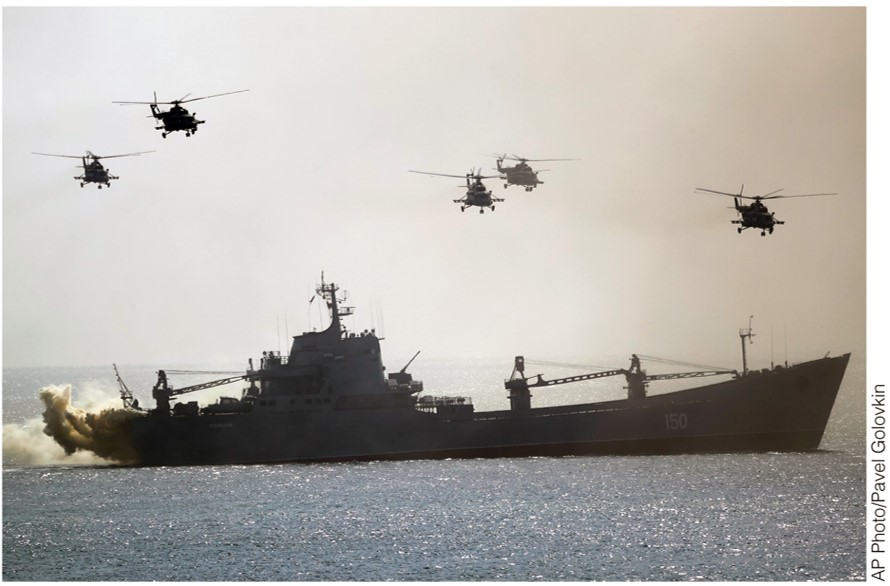
\includegraphics[width=\textwidth,height=0.8\textheight,keepaspectratio]{Russiadrill.jpg}
\end{frame}
%In September 2016, Russia initiated massive military drills, showcasing the country’s ships, cruise missiles, and antiaircraft system, off the coast of Crimea. How much of a country’s capabilities it is willing to mobilize for war can be a source of uncertainty in bargaining.

\begin{frame} 
	\frametitle{\LARGE{Credible Communication Effectiveness}}
So, how effective are these methods? Let's begin with \textbf{brinksmanship}. \pause
	\begin{itemize}
		\item Cuban Missile Crisis is most famous example. \pause
		\\~\\
		\item Hard to identify,except in hindsight. \pause
		\\~\\
		\item Unclear what the difference is between a strategy of brinksmanship and simple aggression or miscalculation of the bargaining range.
	\end{itemize}
\end{frame}

\begin{frame} 
	\frametitle{\LARGE{Credible Communication Effectiveness}}
	What about \textbf{tying hands}? \pause
	\begin{itemize}
		\item Strong support from game theory scholars. \pause
		\\~\\
		\item Conditionality reduces uncertainty by making action and result very clear. \pause
		\\~\\
		\item May be more effective with some (democratic) domestic institutions than others.
	\end{itemize}
\end{frame}

\begin{frame} 
	\frametitle{\LARGE{Credible Communication Effectiveness}}
	What about \textbf{paying for power} and \textbf{sunk costs}? \pause
	\begin{itemize}
		\item Some support for the paying for power: visible military expenditures may make capabilities more clear, reducing private information. \pause
		\begin{itemize}
			\item Weaker support from game theory scholars compared to tying hands. \pause
		\end{itemize}
		\item A sunk costs strategy may be irrational: if an actor deliberately creates sunk costs to demonstrate resolve, why shouldn't an observer conclude that they are now \textit{weaker} due to losing those resources?
	\end{itemize}
\end{frame}

\begin{frame} 
	\frametitle{\LARGE{Information Problems Summary}}
	\begin{itemize}
		\item What prevents states from finding a settlement that both prefer to war?
		\item They both have private information about their capabilities and/or resolve.
		\item They both have incentives to misrepresent that information to get a better deal.
		\item Thus, neither can trust the other's statements, potentially leaving them unable to find a bargaining range they agree on.
		\item States can try to solve this by using strategies for credible communication.
	\end{itemize}
\end{frame}

\begin{frame} 
	\frametitle{\LARGE{Limits of Private Information}}
	\begin{itemize}
		\item Problems of credible communication may explain why wars start, but they become less plausible the longer a war goes on. \pause
		\item \textbf{Why? War itself reveals information about costs and likely outcomes.} \pause
		\item So, what explains wars that have lasted for a long time, or wars where both sides have reliable information on the costs and likely outcome?
	\end{itemize}
\end{frame}

\begin{frame} 
	\frametitle{\LARGE{Commitment Problems}}
	\begin{itemize}
		\item This brings us to the second of Fearon's explanations for war: \textbf{commitment problems}. \pause
		\item These are concerned not with private information, but with whether actors can be trusted to honor an agreement once it is made. \pause
		\begin{itemize}
			\item This means commitment problems can occur even if there is \textit{complete} information on both sides. \pause
			\item Anarchy as a permissive factor is especially important here.
		\end{itemize}
	\end{itemize}
\end{frame}

\begin{frame} 
	\frametitle{\LARGE{Commitment Problems}}
	\begin{itemize}
		\item \textbf{Credible commitment}: a believable agreement by one side to not try to alter the situation after a negotiated settlement is reached. \pause 
		\item A \textbf{commitment problem} occurs when states cannot credibly agree not to threaten or use force to change a negotiated settlement in the future, even if that settlement is acceptable to both of them in the present.
	\end{itemize}
\end{frame}


\begin{frame} 
	\frametitle{\LARGE{Communication vs. Commitments}}
	\begin{itemize}
		\item Note the difference between credible communication and credible commitments. \pause
		\item \textbf{Credible communication}: communicating one's capabilities and/or resolve in a believable way.  
		\begin{itemize}
			\item A solution to the problem of incomplete information. \pause
		\end{itemize}
		\item \textbf{Credible commitment}: a negotiated settlement with terms that neither side will attempt to alter in the future (via force or otherwise). \pause
		\begin{itemize}
			\item Commitment problems occur because making a credible commitment is difficult.
		\end{itemize}
	\end{itemize}
\end{frame}

\begin{frame} 
	\frametitle{\LARGE{Bargaining Over Future Sources of Power}}
	\begin{itemize}
		\item At their core, commitment problems are a form of crisis bargaining over future sources of power. \pause
		\item That is, any negotiated settlement at $t_1$ will reflect the balance of power then. \textbf{But what if that distribution of power changes over time or because of the deal itself}? \pause
		\item In this case, at least one side will no longer have an incentive to honor the deal. But since both sides are rational and can anticipate this, avoiding war becomes more difficult.	
	\end{itemize}
\end{frame}

\begin{frame} 
	\frametitle{\LARGE{Examples of Future Sources of Power}}
	\begin{itemize}
		\Large{
			\item \textbf{Weapons programs}: especially nuclear ones (ex: Iran, North Korea).
			\item\textbf{Strategically valuable territory}: Senkaku/Diaoyu Islands, South China Sea, Golan Heights, oil fields, lucrative shipping lanes, etc.
		}
	\end{itemize}
\end{frame}

\begin{frame} 
	\frametitle{\LARGE{Commitment Problem Types}}
	Bargaining over sources of future power (commitment problems) can take one of two forms:
	\begin{enumerate}
		\item \textbf{Preventive War} 
		\item\textbf{Preemptive War} (also called war with first-strike advantages)
	\end{enumerate}

\end{frame}

\begin{frame} 
	\frametitle{\LARGE{Logic of Preventive War}}
	\begin{itemize}
		\item With incomplete information, we looked at two states bargaining at a single moment in time. 
		\item Now, we shift to these states considering not only the present ($t_1$) but also the future ($t_2$). \pause
		\item \textbf{States have incentives not to bargain over things that diminish their future power.} \pause 
		\item Any rational state will be reluctant to agree to any settlement that will make it vulnerable in the future, even if that settlement is rational in the present.  
	\end{itemize}
\end{frame}

\begin{frame} 
	\frametitle{\LARGE{Logic of Preventive War}}
	\begin{itemize}
		\item If State B makes concessions to avoid war that weaken it today ($t_1$), it cannot be sure that State A will not press for more concessions at $t_2$ now that B is weaker. \pause
		\item Why? \textbf{State A, which will be militarily advantaged by striking this bargain at $t_1$, cannot credibly commit not to exploit the new distribution of power that favors it in $t_2$.}
	\end{itemize}
\end{frame}

\begin{frame} 
	\frametitle{\LARGE{Logic of Preventive War}}
	\begin{itemize}
		\item Another way to phrase this is to say that State B is undergoing a \textbf{power shift}: a  change in the distribution of power between these two states. State A (the ``rising power") is growing stronger while state B is growing weaker. \pause
		\item When the distribution of power is anticipated to change rapidly, states have incentives to initiate \textbf{preventive war}: war fought due to anticipation of a rival state becoming stronger in the future.  
	\end{itemize}
\end{frame}

\begin{frame} 
	\frametitle{\LARGE{Logic of Preventive War}}
	\begin{itemize}
		\item Under the bargaining model of war, a rising power has an incentive to alter the status quo in the future ($t_2$) once it is powerful enough to do so. \pause
		\item Knowing this, its opponents have incentives to attack it while it is currently weak (at $t_1$). \pause 
		\item Example: Iraq War (according to US)
	\end{itemize}
\end{frame}

\begin{frame} 
	\frametitle{\LARGE{Today ($t_1$): B is Relatively Strong}}
	\begin{figure}[ht!]
		\centering
		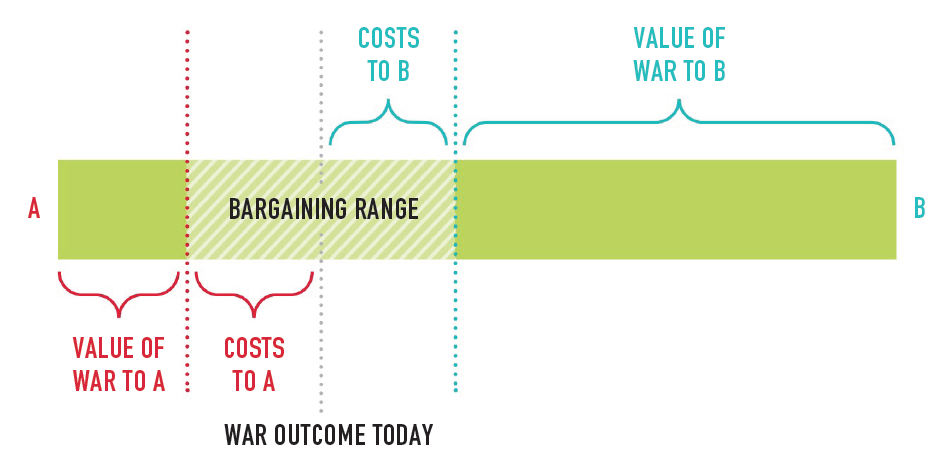
\includegraphics[width=\textwidth,height=0.8\textheight,keepaspectratio]{./cred1.png}
	\end{figure}
\end{frame}

\begin{frame} 
	\frametitle{\LARGE{Tomorrow ($t_2$): B is Relatively Weak}}
	\begin{figure}[ht!]
		\centering
		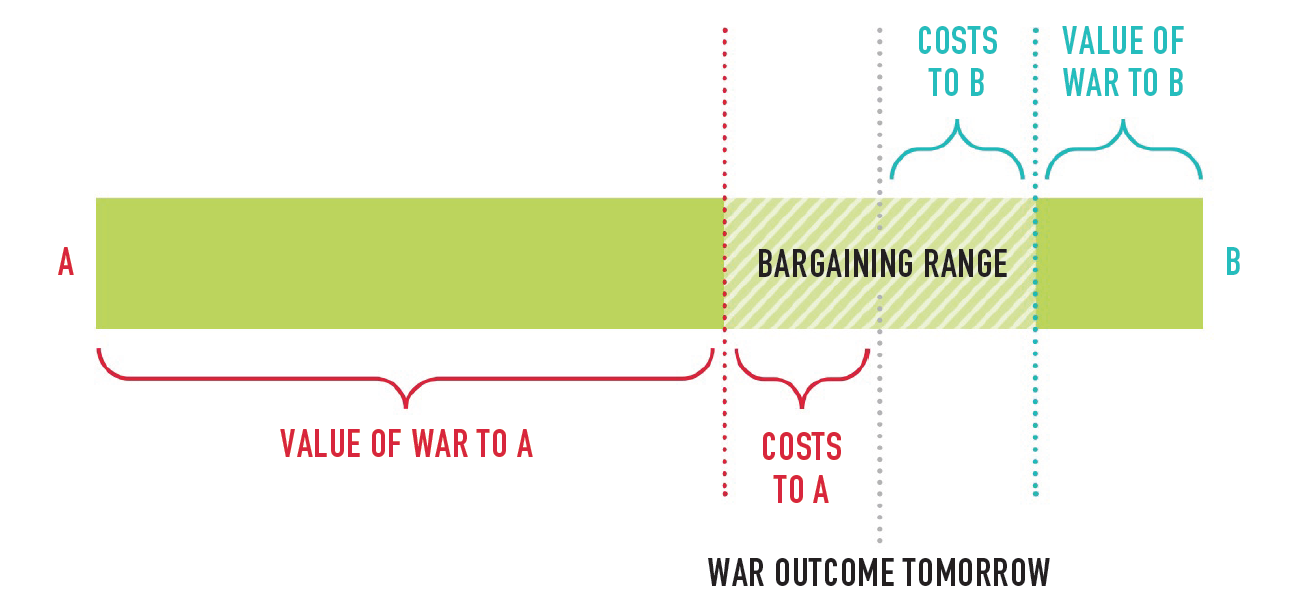
\includegraphics[width=\textwidth,height=0.8\textheight,keepaspectratio]{./cred2.png}
	\end{figure}
\end{frame}

\begin{frame} 
	\frametitle{\LARGE{Preventive Wars}}
	\begin{itemize}
		\item A preventive war is fought because a rational state would rather fight a weak rival today than a strong rival tomorrow. \pause
		\item Why can't the rising power promise not to abuse its new power? \pause \textbf{Because the incentive structures of the situation, and lack of enforcement mechanisms for any deal, give it every incentive to renege on any deal.}
	\end{itemize}
\end{frame}

\begin{frame} 
	\frametitle{\LARGE{Preventive Wars}}
	\begin{itemize}
		\item This change in power can occur for a variety of reasons. \pause
		\begin{itemize}
			\item An economic deal that disproportionately benefits one side. \pause
			\item Growth in one side's military strength due to technological or other advances. \pause
			\item An impending alliance deal (ex: what if Ukraine joined NATO?). \pause
			\item Any present deal that cedes strategic territory to the other side (ex: appeasement)
		\end{itemize}
		\item This change in power can also take two general forms...
	\end{itemize}
\end{frame}

\begin{frame} 
	\frametitle{\LARGE{Rapidly Growing Power}}
	\begin{figure}[ht!]
		\centering
		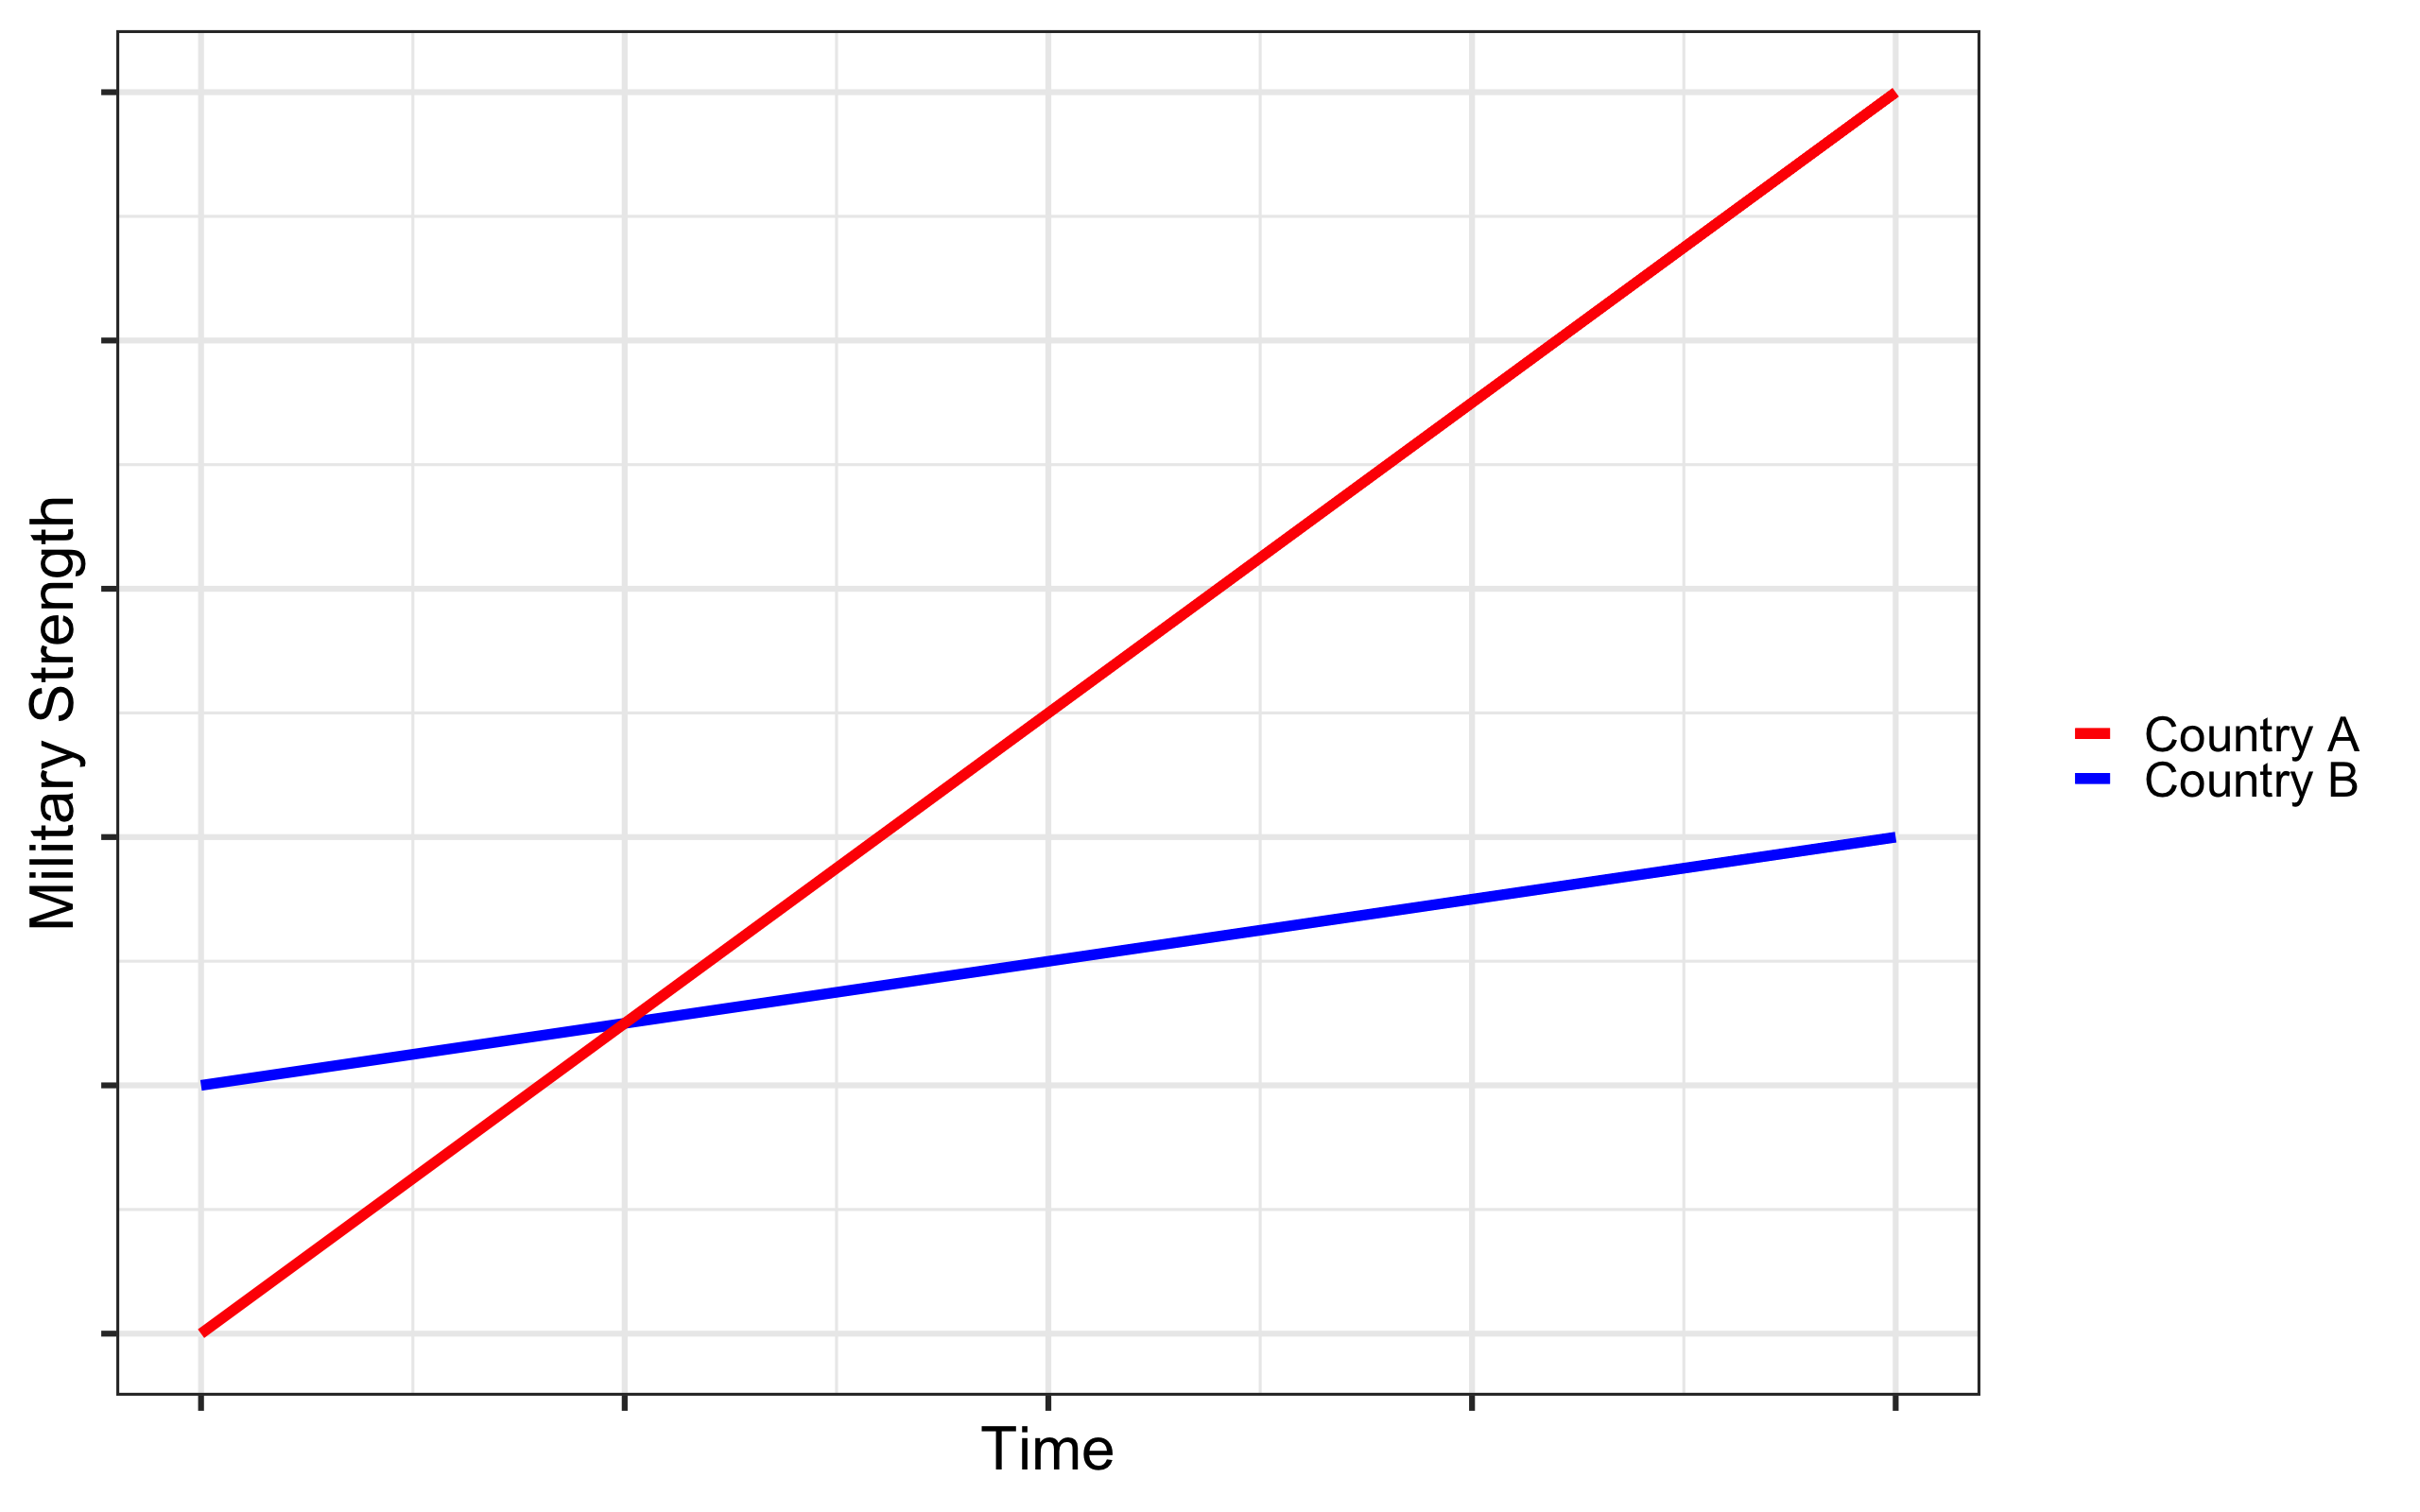
\includegraphics[height=.85\textheight, keepaspectratio]{./rapid_growth.png}
	\end{figure}
\end{frame}

%pic from https://www.britannica.com/event/Pearl-Harbor-attack
\begin{frame} 
	\frametitle{\LARGE{Example: Pearl Harbor}}
	\begin{figure}[ht!]
		\centering
		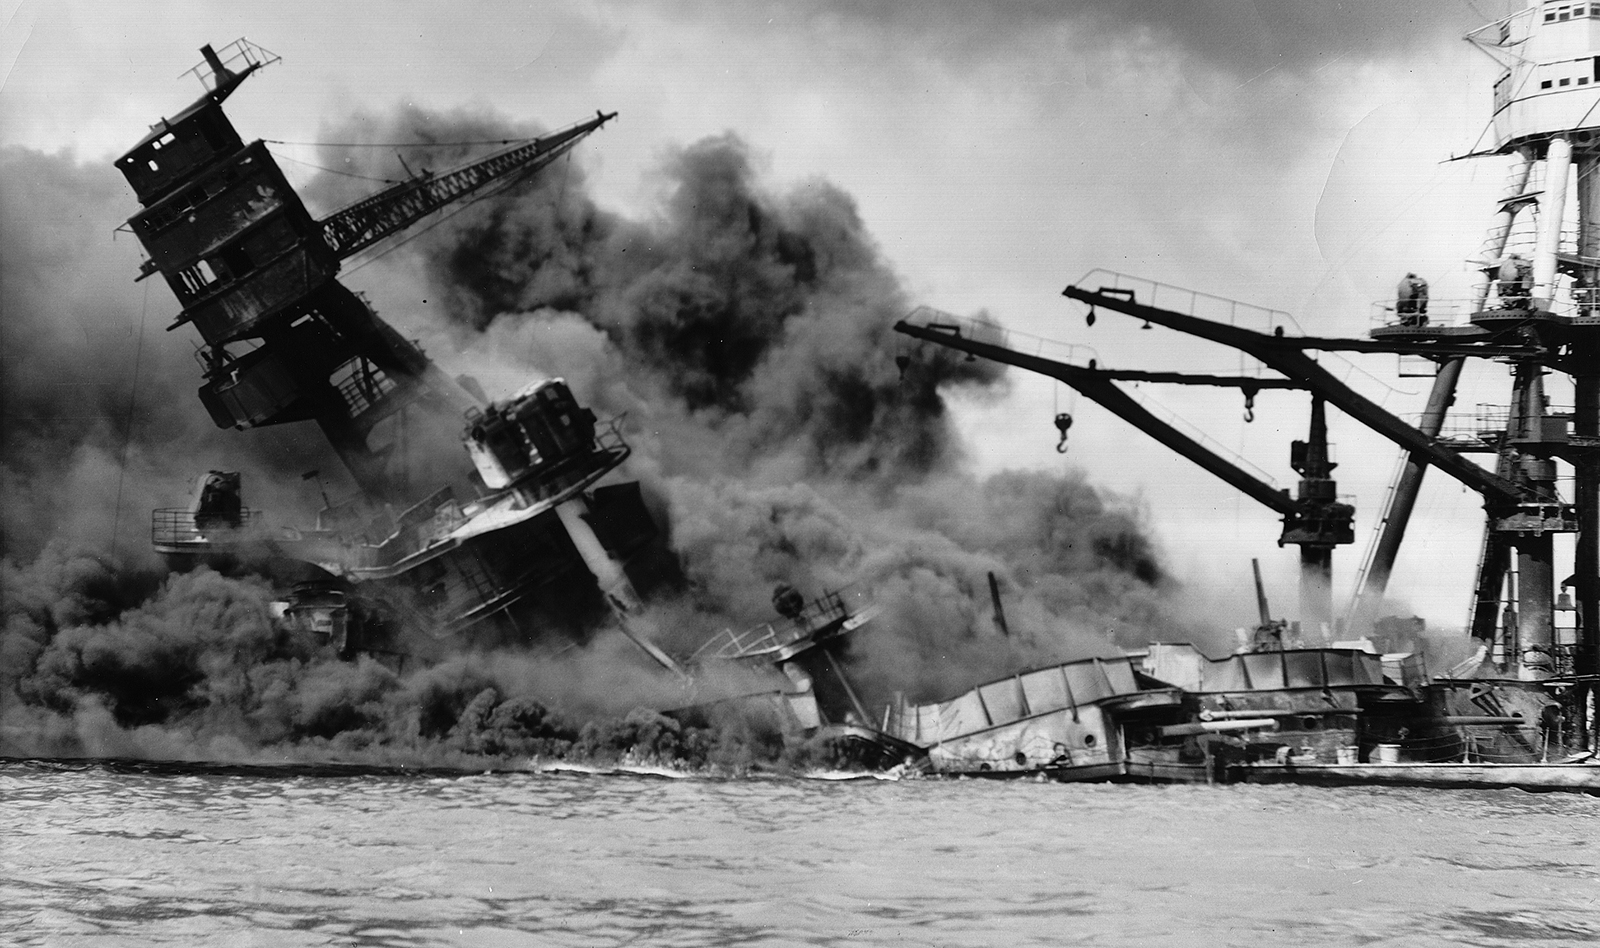
\includegraphics[height=.9\textheight, keepaspectratio]{Pearlharbor.jpg}
	\end{figure}
\end{frame}

%https://www.abc.net.au/science/articles/2003/03/17/808818.htm
%book by Bennet and Stam 2003, The Behavioural Origins of War: Cumulation and Limits to Knowledge in Understanding International Conflict. 
\begin{frame} 
	\frametitle{\LARGE{Example: Pearl Harbor}}
	\begin{itemize}
		\item Japanese actions against China in the 1930s lead to retaliatory US trade restrictions. \pause
		\item American trade restrictions on oil and steel hurt Japan's military. \pause
		\item Japanese government fears that continued restrictions will further weaken them. \pause
		\item Thus, Japanese government concludes they would rather fight a (relatively) weaker US today than wait for the balance of power to disadvantage them even further.
	\end{itemize}
\end{frame}

\begin{frame} 
	\frametitle{\LARGE{Discontinuous Shift in Power}}
	\begin{figure}[ht!]
		\centering
		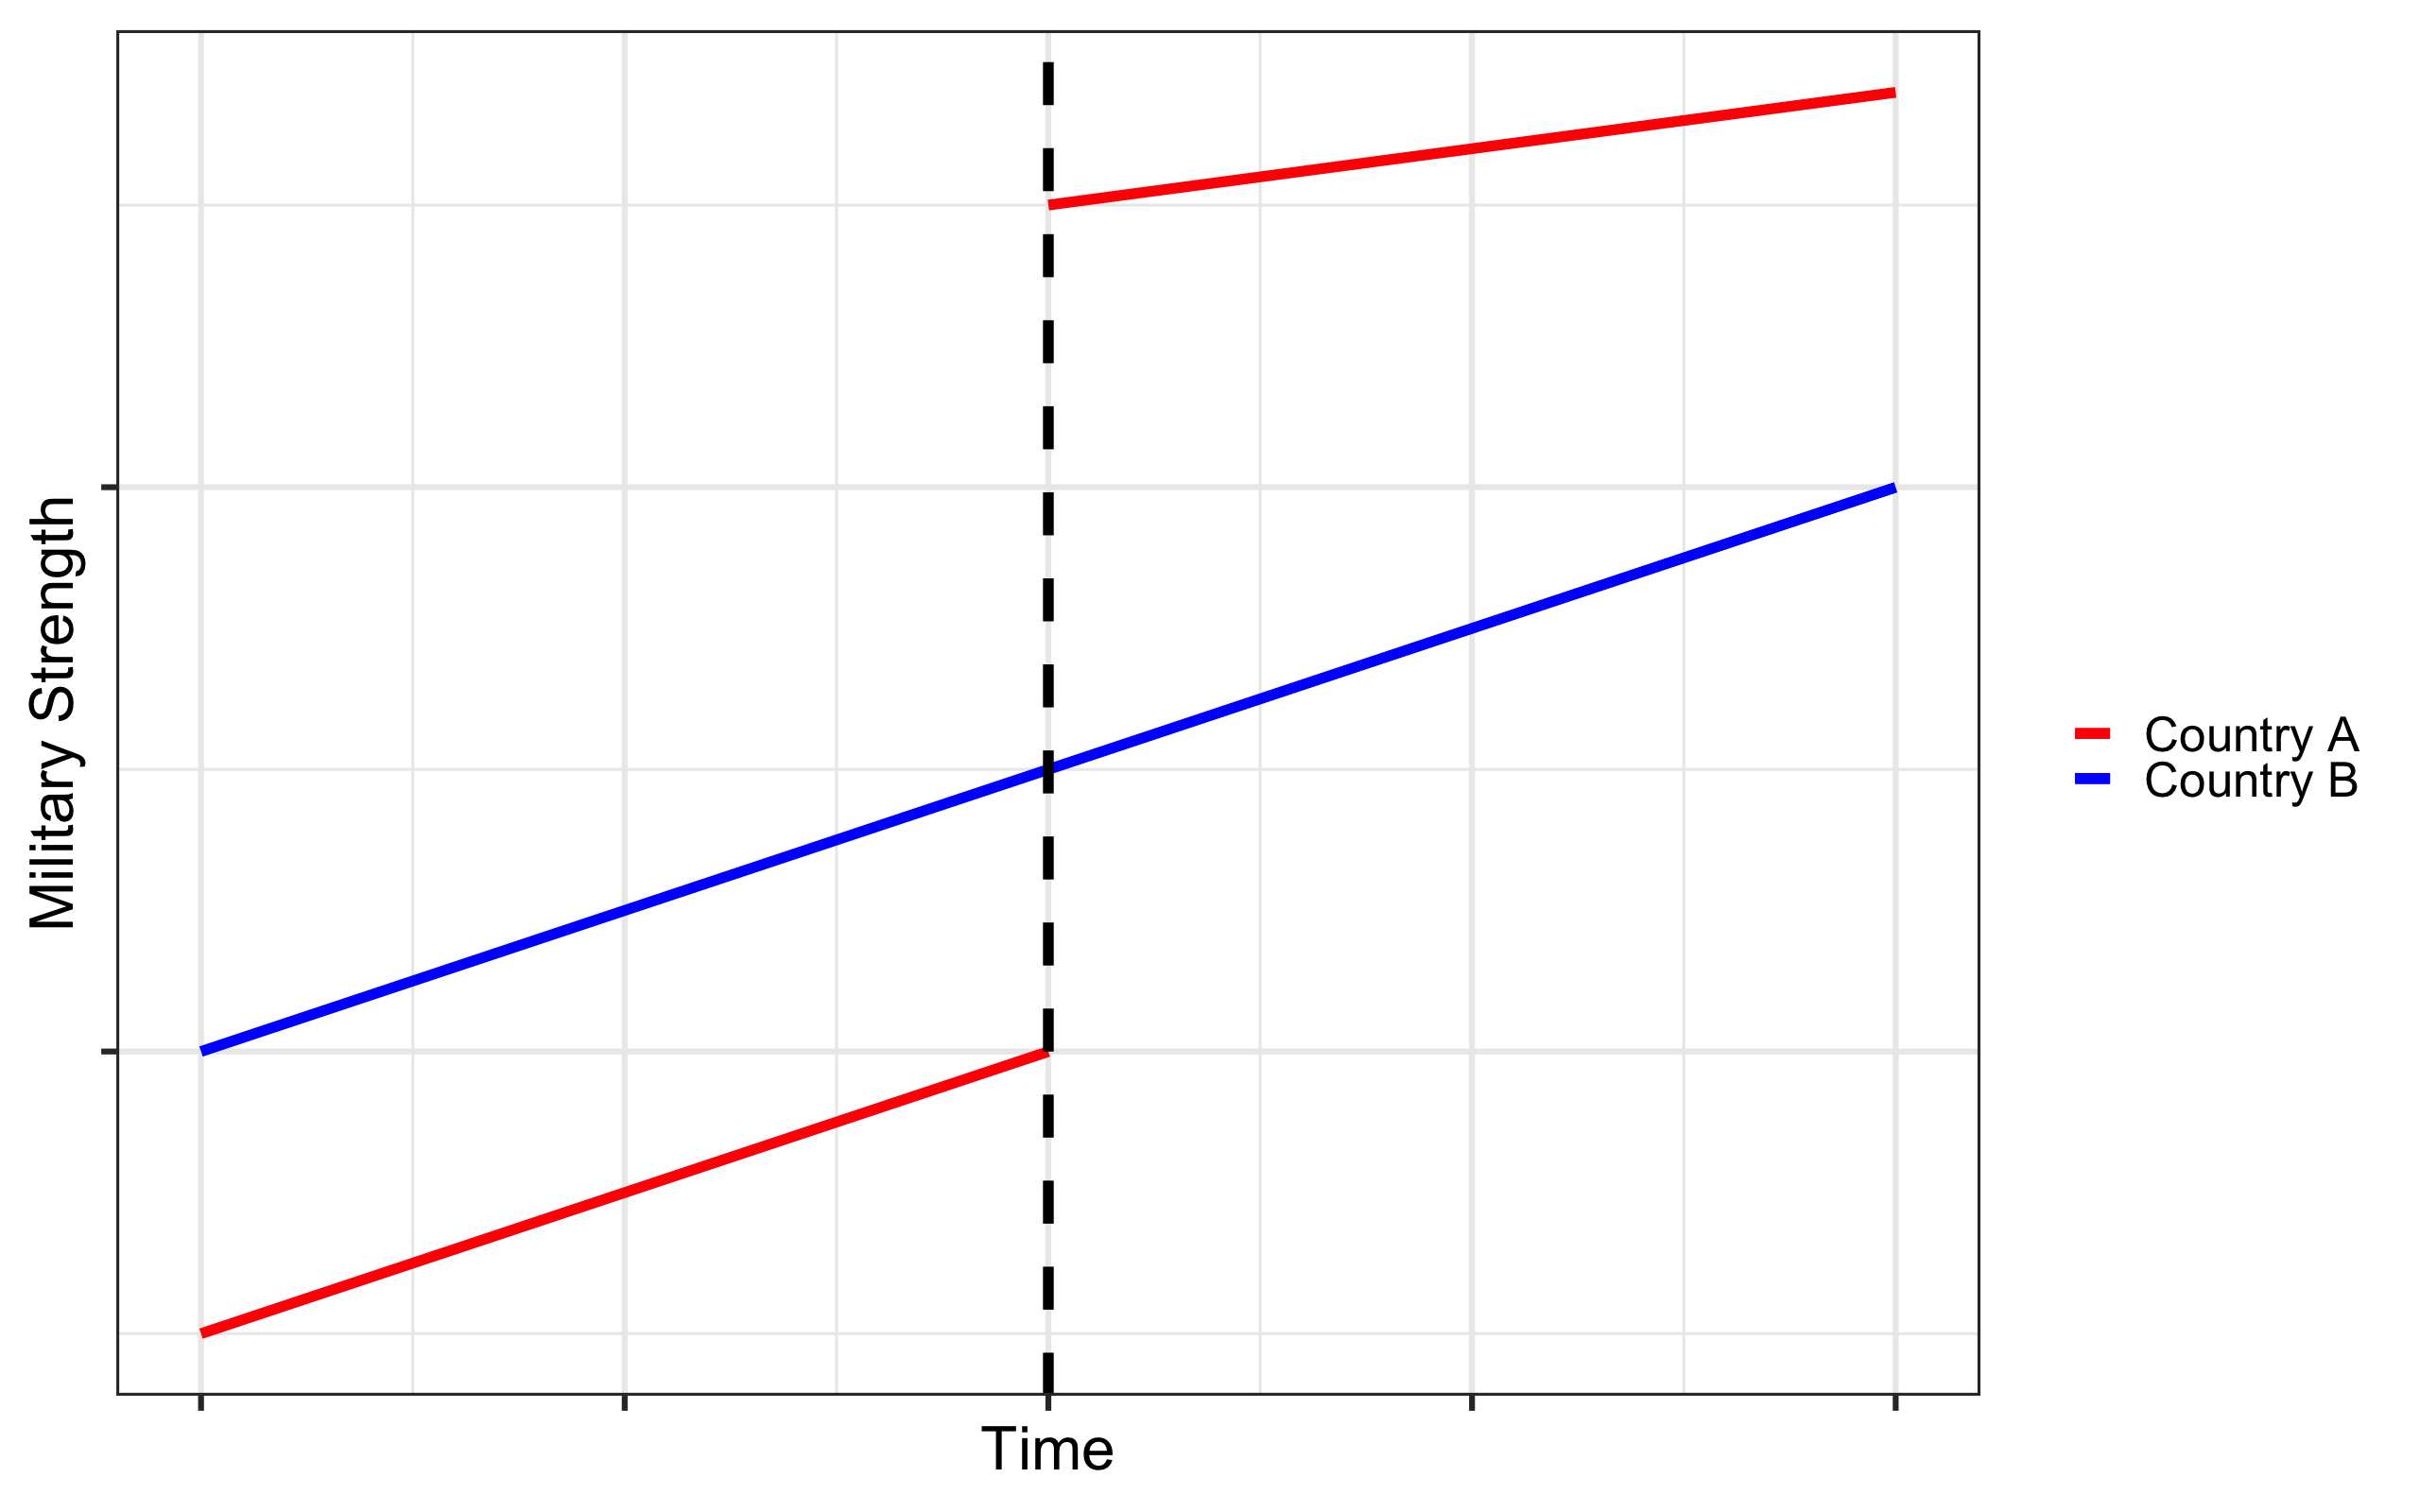
\includegraphics[height=.85\textheight, keepaspectratio]{./disc_jump.png}
	\end{figure}
\end{frame}

%pic from https://www.msnbc.com/andrea-mitchell/10-years-ago-today-saddam-hussein-statue-top-msna56149
%pic from https://www.britannica.com/event/Pearl-Harbor-attack
\begin{frame} 
	\frametitle{\LARGE{Example: US Invasion of Iraq in 2003}}
	\begin{figure}[ht!]
		\centering
		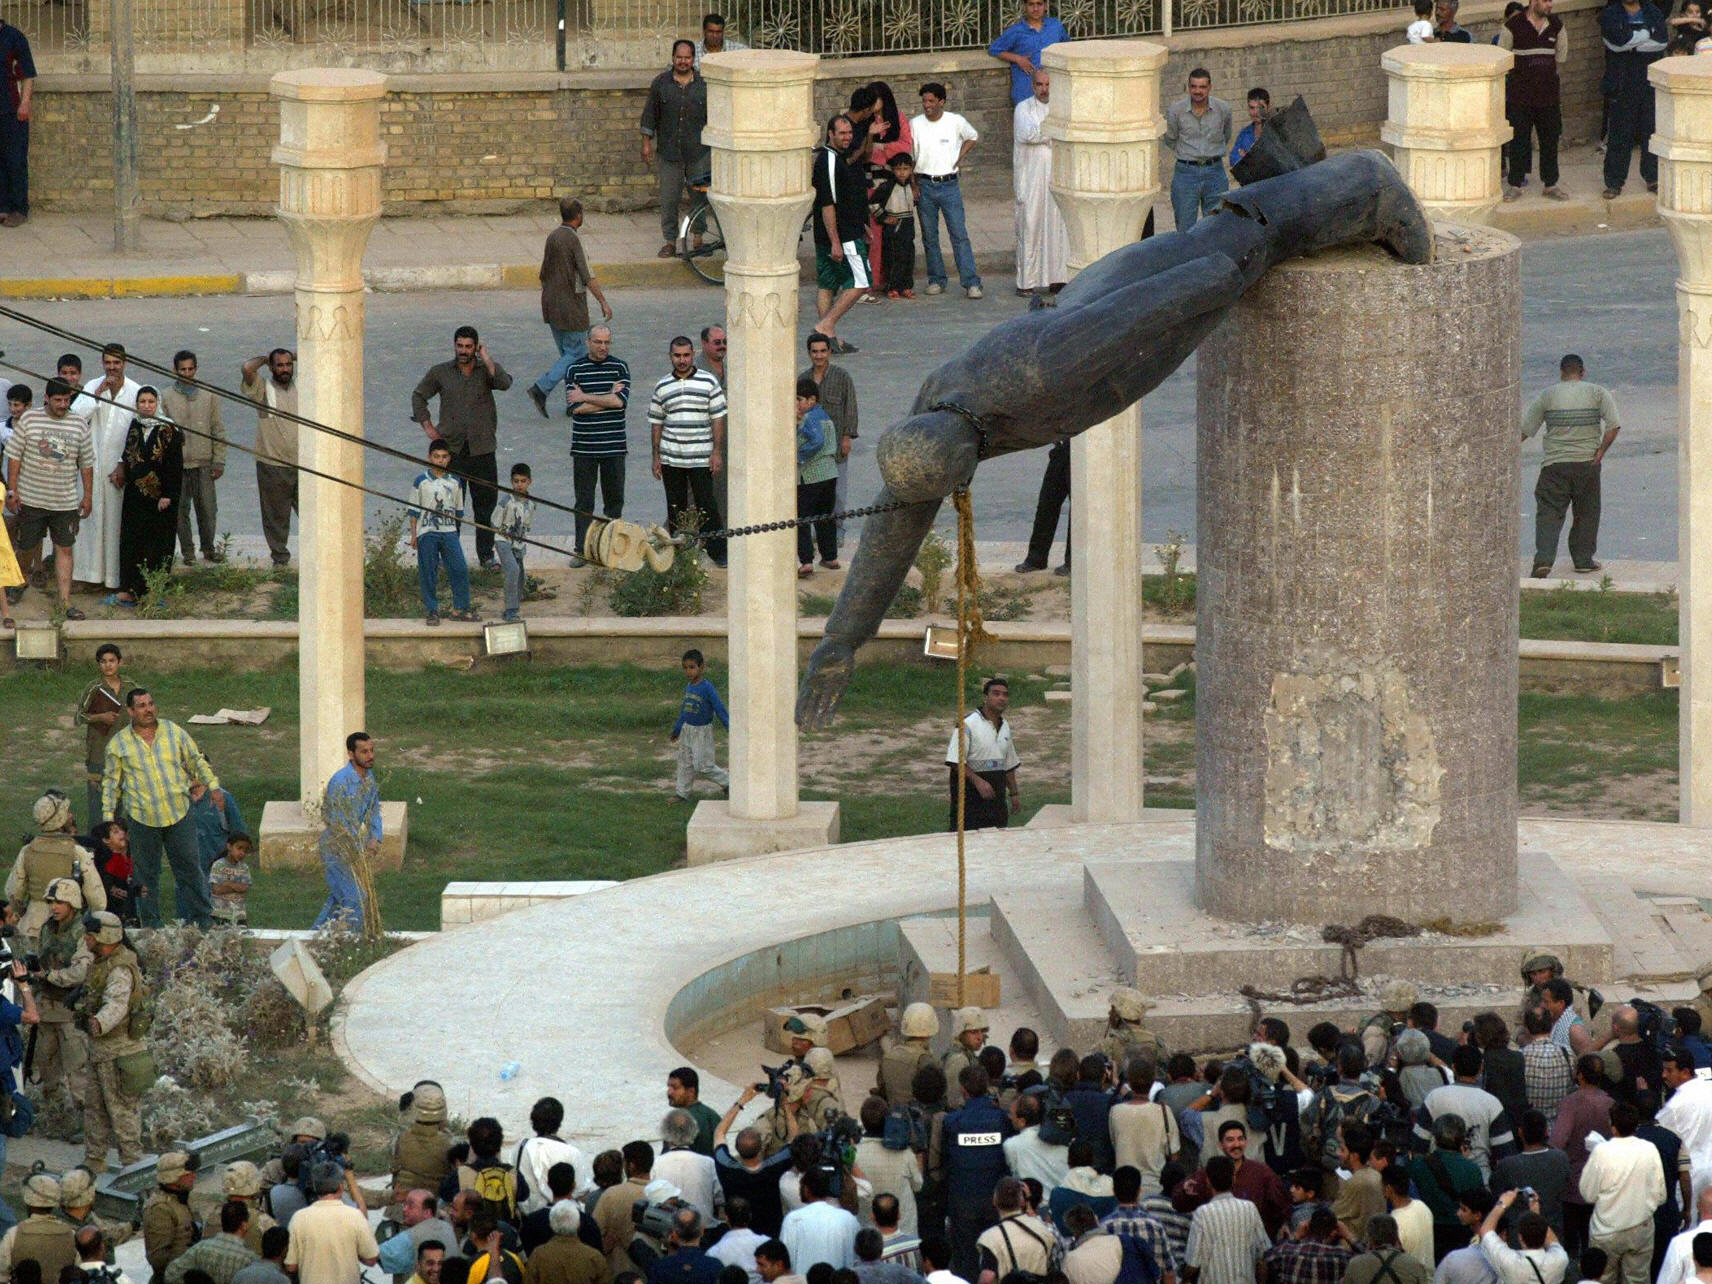
\includegraphics[height=.9\textheight, keepaspectratio]{Saddamstatue.jpg}
	\end{figure}
\end{frame}

\begin{frame} 
	\frametitle{\LARGE{Example: US Invasion of Iraq in 2003}}
	\begin{itemize}
		\item American justification for the invasion was that Iraq was developing WMDs, supporting terrorist groups (including AQ), committing human rights abuses. \pause
		\item Most important part of this justification was the purported WMD program. \pause
		\item Development of working WMDs represents a discontinuous shift in power. \pause
		\item No WMDs ever found, nor any evidence that Saddam was working with AQ...
	\end{itemize}
\end{frame}


\begin{frame} 
	\frametitle{\LARGE{Preemptive War}}
	\begin{itemize}
		\item The second subtype of commitment problem involves the possibility of \textbf{preemptive war}: war with first-strike advantages. \pause
		\item States have a \textbf{first-strike advantage} when there is a significant military benefit to being the first to attack. \pause
		\begin{itemize}
			\item Ex: nuclear first-strike advantage (prior to development of second-strike capabilities).
		\end{itemize}
		\item If a state fears that the other side will attack first, and there is a first-strike advantage, it has incentives to preempt that attack by launching its own. \pause 
		\begin{itemize}
			\item Ex: Israel during the Six-Day War
		\end{itemize}
		\item Shares similarities with the Prisoner's Dilemma...
	\end{itemize}
\end{frame}

\begin{frame} 
	\frametitle{\LARGE{State A Attacks First}}
	\begin{figure}[ht!]
		\centering
		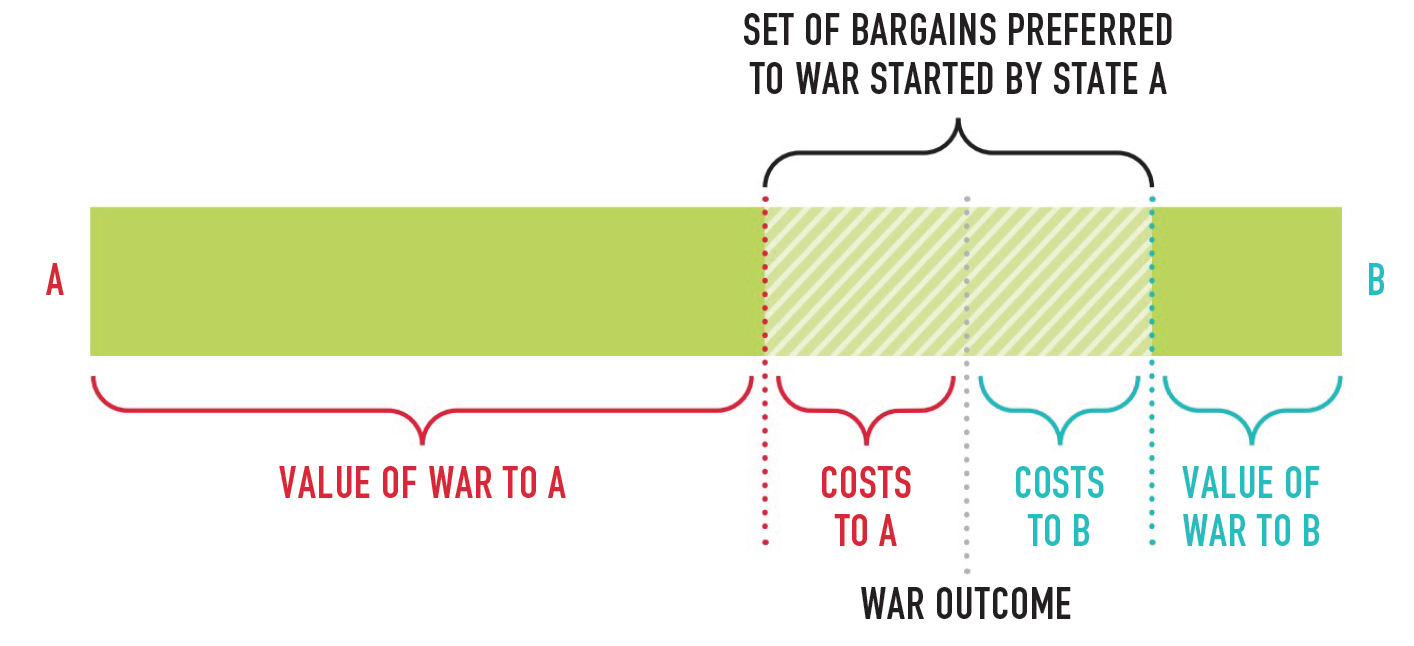
\includegraphics[width=\textwidth,height=0.8\textheight,keepaspectratio]{./stateafirst.png}
	\end{figure}
\end{frame}

\begin{frame} 
	\frametitle{\LARGE{State B Attacks First}}
	\begin{figure}[ht!]
		\centering
		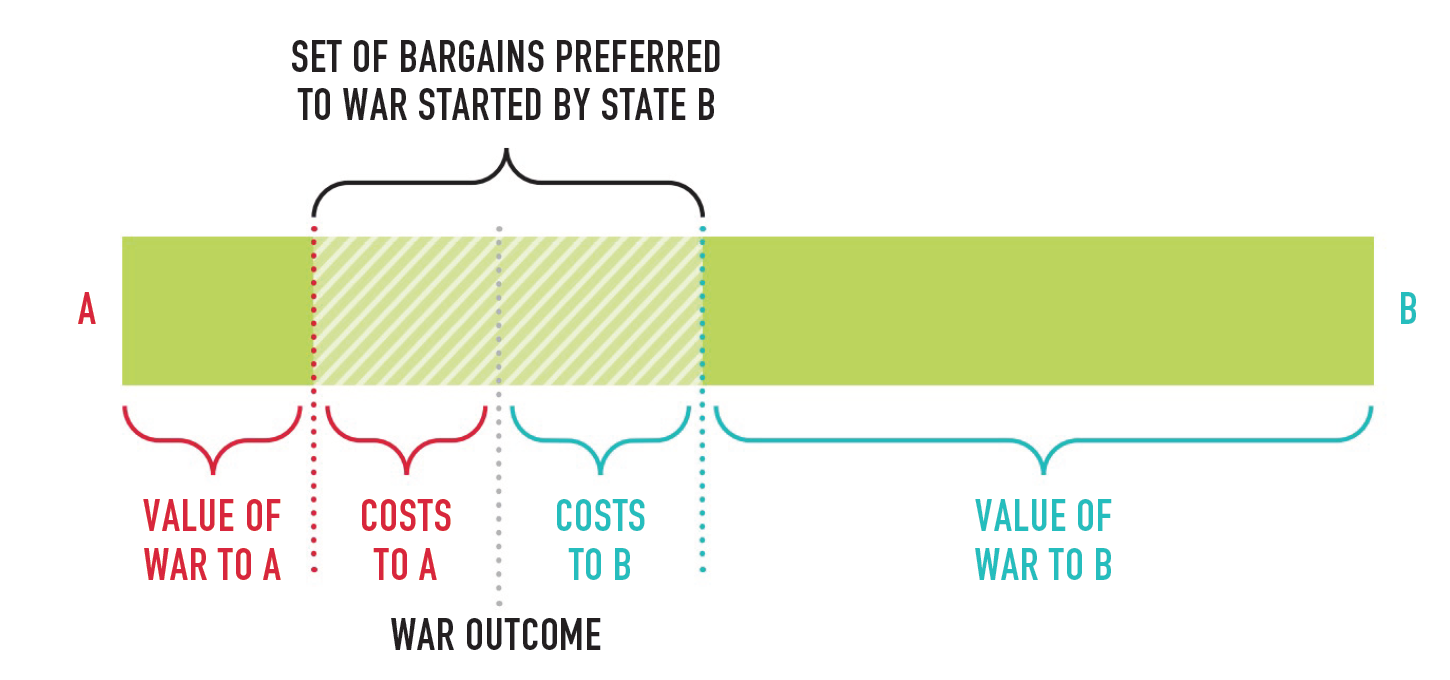
\includegraphics[width=\textwidth,height=0.8\textheight,keepaspectratio]{./statebfirst.png}
	\end{figure}
\end{frame}

%pic from https://www.irishtimes.com/news/world/middle-east/how-the-six-day-war-turned-israel-into-regional-superpower-1.3112468
\begin{frame} 
	\frametitle{\LARGE{Example: 1967 Six-Day War}}
	\begin{figure}[ht!]
		\centering
		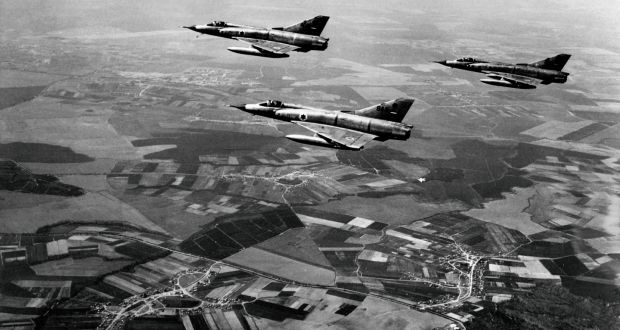
\includegraphics[width=\textwidth,height=0.8\textheight,keepaspectratio]{IsraelAF.jpg}
	\end{figure}
\end{frame}

\begin{frame} 
	\frametitle{\LARGE{Example: 1967 Six-Day War}}
	\begin{itemize}
		\item Background: escalating tensions between Israel and Egypt over strategic territory (Straits of Tiran - vital shipping corridor). \pause
		\item Egypt mobilizes its forces and ejects UN peacekeepers from the Israel-Egypt border. \pause
		\item Israeli air force preemptively strikes Egyptian air force, catching it completely by surprise. \pause
		\item Egyptian air force crippled; Israel routs Egypt and its allies Syria and Jordan.
	\end{itemize}
\end{frame}

\begin{frame} 
	\frametitle{\LARGE{Commitment Problems and War Length}}
	\begin{itemize}
		\item Weisiger (2016) examines 103 interstate wars since 1816. \pause
		\item Wars due to incomplete information tend to be short because during the war previously private information becomes public. Under reduced uncertainty, it is easier to strike a bargain. \pause
		\item Wars stemming from commitment problems tend to last longer. \pause
		\item The longest wars have been fought between declining and rising states when preventive war motivations are strong.  
	\end{itemize}
\end{frame}

\begin{frame} 
	\frametitle{\LARGE{War Duration}}
	\begin{figure}[ht!]
		\centering
		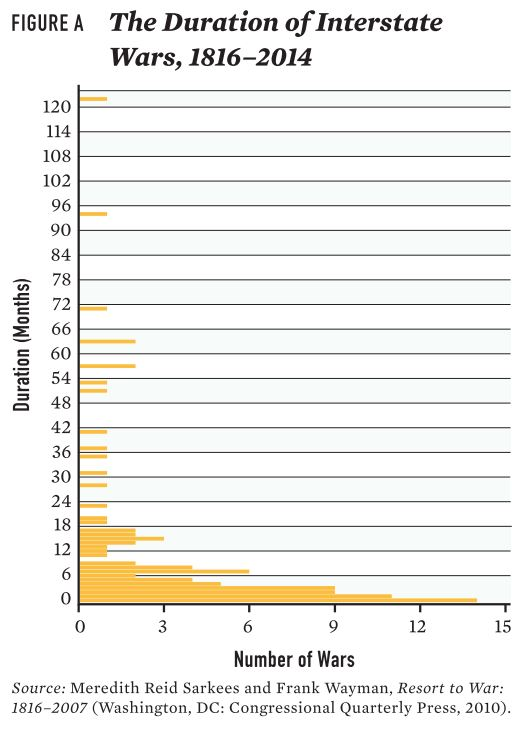
\includegraphics[width=\textwidth,height=0.8\textheight,keepaspectratio]{war duration.JPG}
	\end{figure}
\end{frame}

\begin{frame} 
	\frametitle{\LARGE{Commitment Problem Solutions}}
	\begin{itemize}
		\item Solutions generally focus on finding a third party to guarantee a deal. \pause
		\item If a third party can prevent one side from taking advantage of its shift in power, then the other side may not feel the need to engage in preventive or preemptive war. \pause
		\item Frequently accomplished via use of UN peacekeeping forces, in cases that involve territory (ex: UN forces in Golan Heights between Israel and Syria). \pause
		\item Peacekeepers serve as both deterrent and early warning mechanism, decreasing uncertainty.
	\end{itemize}
\end{frame}

\begin{frame} 
	\frametitle{\LARGE{War Due to Indivisibility}}
	\begin{itemize}
		\item Thus far, we have assumed that the crisis bargaining is over some \textbf{divisible good}: a good that can, in theory, be divided.
		\item Territory has been our go-to example, but other divisible goods exist (policy choices, economic treaties, etc.)
		\item However, some goods cannot be divided without substantially diminishing or destroying their values. These are \textbf{indivisible goods}. \pause
		\begin{itemize}
			\item Ex: 100 pennies versus \$1 dollar bill
		\end{itemize}
	\end{itemize}
\end{frame}

\begin{frame} 
	\frametitle{\LARGE{Indivisibility}}
	\begin{itemize}
		\item Bargaining breakdown will occur if states are bargaining over an indivisible good. \pause
		\item Why? \textbf{By definition, such a good cannot be divided, meaning any bargain will involve one side getting all of it. This will be unacceptable to the other side.}
		\item Most commonly cited example is Jerusalem. 
	\end{itemize}
\end{frame}

%\begin{frame} 
%	\frametitle{\LARGE{Indivisiblity: Jerusalem}}
%	\begin{figure}[ht!]
%		\centering
%		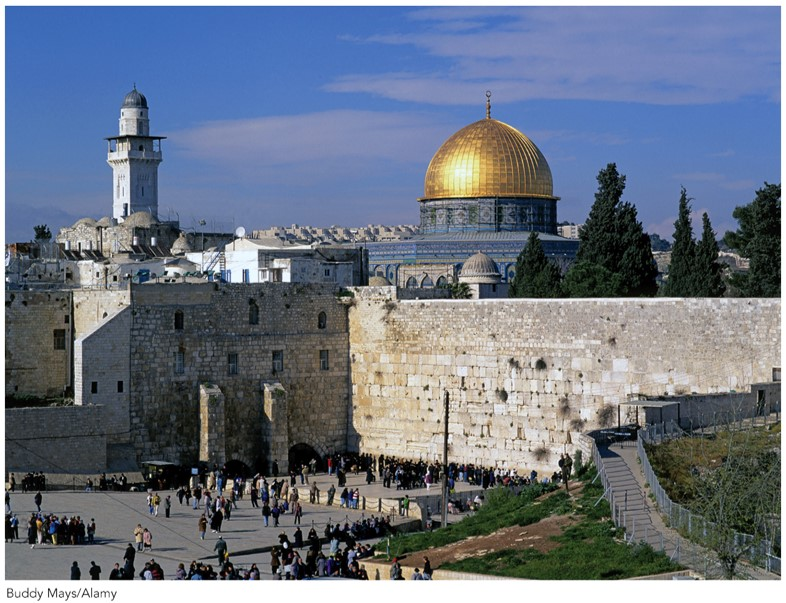
\includegraphics[width=\textwidth,height=0.8\textheight,keepaspectratio]{Jerusalem.jpg}
%	\end{figure}
%\end{frame}

\begin{frame} 
	\frametitle{\LARGE{Indivisibility}}
	\begin{itemize}
		\item But should we be skeptical that indivisible goods exist? \pause 
		\begin{itemize}
			\item Weak enforcement mechanisms may cause actors to claim indivisibility when the real issue is commitment. \pause 
			\item States have bargaining incentives to claim indivisibility. \pause 
			\item Indivisibility can be socially constructed (ex: 1950s Jerusalem UN control proposals).
		\end{itemize}
	\end{itemize}
\end{frame}

\begin{frame} 
	\frametitle{\LARGE{Indivisibility Solutions}}
	Some solutions have been proposed:
	\begin{itemize}
		\item \textbf{Shared control}: both sides keep control of the valuable good. \pause \\~\\
		\item \textbf{Issue linkage}: one side gets everything they want on one issue, while ceding another issue to the other side. \pause 
	\end{itemize}
	Neither of these solutions strictly work within the confines of Fearon's rational model, but both are plausible.
\end{frame}

\begin{frame} 
	\frametitle{\LARGE{South China Sea}}
	\begin{figure}[ht!]
		\centering
		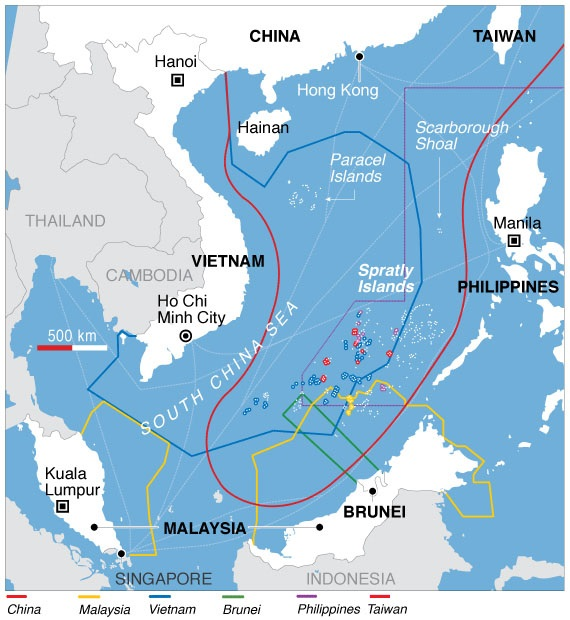
\includegraphics[width=\textwidth,height=0.8\textheight,keepaspectratio]{South_China_Sea_claims_map.jpg}
	\end{figure}
\end{frame}

\begin{frame} 
	\frametitle{\LARGE{South China Sea}}
	\begin{itemize}
		\item What do the points raised in the Mastro article tell us? \pause
		\item Actual conflicts are generally far more complicated than two-player models suggest. \pause
		\begin{itemize}
			\item Multiple players, multiple simultaneous crisis bargaining interactions... \pause
		\end{itemize}
		\item Information and commitment problems abound, often at the same time. \pause  
		\begin{itemize}
			\item What about indivisibility? \pause
		\end{itemize}
		\item Both the US and China are struggling with issues of credible signalling and future sources of power. \pause 
		\item Do the US policies Mastro proposes address the heart of the bargaining issue? 
	\end{itemize}
\end{frame}

\begin{frame} 
	\frametitle{\LARGE{Is Interstate War Obsolete?}}
	\begin{itemize}
		\item The bargaining model proposes three features of war: \pause 
		\begin{enumerate}
			\item Conflicting interests  
			\item Costs of war  
			\item Bargaining failure because of information, commitment, or indivisibility problems \pause
		\end{enumerate}
		\item Some scholars have argued that changes in the international system have impacted these features, making interstate war obsolete.
	\end{itemize}
\end{frame}

\begin{frame} 
	\frametitle{\LARGE{Is Interstate War Obsolete?}}
	These changes include:
	\begin{itemize}
		\item International organizations: development of more IOs can decrease private information and help with commitment problems. \pause
		\begin{itemize}
			\item They can decrease private information by providing neutral observers of a state’s military activities.
			\item They can make it easier to resolve commitment problems by monitoring and enforcing agreements.
		\end{itemize}
	\end{itemize}
\end{frame}

\begin{frame} 
	\frametitle{\LARGE{Is Interstate War Obsolete?}}
	These changes also include:
	\begin{itemize}
		\item Spread of democracy: ``democratic peace" makes war less likely in the aggregate as the number of democracies increases.
		\item Increased costs as technology advances (especially nuclear weapons). \pause
		\item Decreased interest in claiming territory. \pause
		\item Globalization and increased economic interdependence raise costs of war. \pause
	\end{itemize}
	Ultimately, all of this explains why interstate wars are rare, but ``obsolete" is probably too strong a term.
\end{frame}


\begin{frame} 
	\frametitle{\LARGE{Bargaining Summary 1}}
	\begin{itemize}
		\item The central puzzle of the bargaining model: why do states fight rather than reaching a negotiated settlement, given the costs of war. \pause 
		\item Explanations:
		\begin{enumerate}
			\item Private information and incentives to misrepresent it \pause
			\item Credible commitment problems \pause
			\item Indivisibility issues (even if socially constructed) 
		\end{enumerate}
	\end{itemize}
\end{frame}

\begin{frame} 
	\frametitle{\LARGE{Bargaining Summary 2}}
	\begin{itemize}
		\item Averting war means finding ways to solve each of these problems. 
		\begin{enumerate}
			\item Decrease private info via tying hands and promoting transparent communication. \pause
			\item Find ways to enforce commitments (often via third parties like IOs) \pause
			\item Address indivisibility issues with linkage or power sharing. \pause
		\end{enumerate}
		\item Increasing the costs of war also works in most cases.
	\end{itemize}
\end{frame}

\begin{frame} 
	\frametitle{\LARGE{Final Thoughts}}
	\begin{itemize}
		\item This provides an answer to a pivotal question of political science: why war? \pause
		\item These explanations can be applied to most interstate conflicts. \pause
		\item Do you find this collection of explanations to be a satisfying theory of interstate conflict?
		\item What is it missing?
	\end{itemize}
\end{frame}

\end{document}
